\documentclass[border=5pt]{standalone}

\usepackage{tikz}
\usetikzlibrary{
    positioning, arrows.meta, calc, backgrounds,
    decorations.markings, decorations.pathmorphing,
    fit, shapes.geometric, patterns, matrix,
    shadows.blur, fadings
}

\usepackage{amsmath, amssymb}
\usepackage{xcolor}
\usepackage[T1]{fontenc}
\usepackage{helvet}
\renewcommand{\familydefault}{\sfdefault}

% ============================================
% NATURE-STYLE PALETTE
% ============================================
\definecolor{nprimary}{HTML}{0077B6}
\definecolor{nprimarydk}{HTML}{023E8A}
\definecolor{naccent}{HTML}{F77F00}
\definecolor{naccentdk}{HTML}{D62828}
\definecolor{ngreen}{HTML}{2D6A4F}
\definecolor{npurple}{HTML}{7209B7}
\definecolor{ngray}{HTML}{6C757D}
\definecolor{ngraylt}{HTML}{E9ECEF}
\definecolor{nbg}{HTML}{FFFFFF}
\definecolor{ntext}{HTML}{212529}
\definecolor{ntextsub}{HTML}{6C757D}

% ============================================
% STYLES
% ============================================
\tikzset{
    module3d/.style={
        rectangle, rounded corners=3pt,
        minimum height=8mm, minimum width=22mm,
        draw=#1!70, line width=0.5pt,
        top color=#1!15, bottom color=#1!35,
        font=\fontsize{7}{8}\selectfont\sffamily,
        drop shadow={shadow xshift=0.5mm, shadow yshift=-0.5mm, opacity=0.2}
    },
    modulebig/.style={
        rectangle, rounded corners=4pt,
        minimum height=10mm, minimum width=28mm,
        draw=#1!80, line width=0.6pt,
        top color=#1!12, bottom color=#1!30,
        font=\fontsize{8}{9}\selectfont\sffamily\bfseries,
        drop shadow={shadow xshift=0.6mm, shadow yshift=-0.6mm, opacity=0.25}
    },
    cellsm/.style={
        circle, minimum size=3mm,
        inner color=#1!25, outer color=#1!65,
        draw=#1!75, line width=0.3pt
    },
    recvcell/.style={
        circle, minimum size=5mm,
        inner color=naccent!40, outer color=naccent!85,
        draw=naccentdk, line width=0.6pt,
        drop shadow={shadow xshift=0.4mm, shadow yshift=-0.4mm, opacity=0.3}
    },
    panel/.style={
        rectangle, rounded corners=5pt,
        fill=white, draw=ngraylt, line width=0.4pt,
        drop shadow={shadow xshift=0.8mm, shadow yshift=-0.8mm, opacity=0.1}
    },
    subpanel/.style={
        rectangle, rounded corners=3pt,
        top color=ngraylt!20, bottom color=ngraylt!50,
        draw=ngraylt!80, line width=0.3pt
    },
    flowarrow/.style={
        -{Stealth[length=2.5mm, width=1.6mm, round]},
        line width=0.7pt, draw=#1
    },
    flowthick/.style={
        -{Stealth[length=3mm, width=2mm, round]},
        line width=1pt, draw=#1
    },
    flowdash/.style={
        -{Stealth[length=2mm, width=1.4mm, round]},
        line width=0.6pt, draw=#1, dashed, dash pattern=on 2.5pt off 1.5pt
    },
    heading/.style={font=\fontsize{9}{10}\selectfont\bfseries\sffamily, text=ntext},
    subhead/.style={font=\fontsize{7}{8}\selectfont\sffamily, text=ntextsub},
    caption/.style={font=\fontsize{6}{7}\selectfont\sffamily, text=ntextsub},
    dimbadge/.style={
        rectangle, rounded corners=1.5pt,
        fill=#1!12, draw=#1!45, line width=0.25pt,
        font=\fontsize{5.5}{6}\selectfont\sffamily,
        inner xsep=2pt, inner ysep=1pt
    },
    eqbox/.style={
        rectangle, rounded corners=2pt,
        fill=ngraylt!40, draw=ngraylt!80, line width=0.3pt,
        inner sep=3pt, font=\fontsize{6.5}{7.5}\selectfont
    },
    secletter/.style={
        circle, minimum size=5mm,
        fill=#1!15, draw=#1!50, line width=0.4pt,
        font=\fontsize{8}{9}\selectfont\bfseries\sffamily, text=#1!70
    },
}

\begin{document}

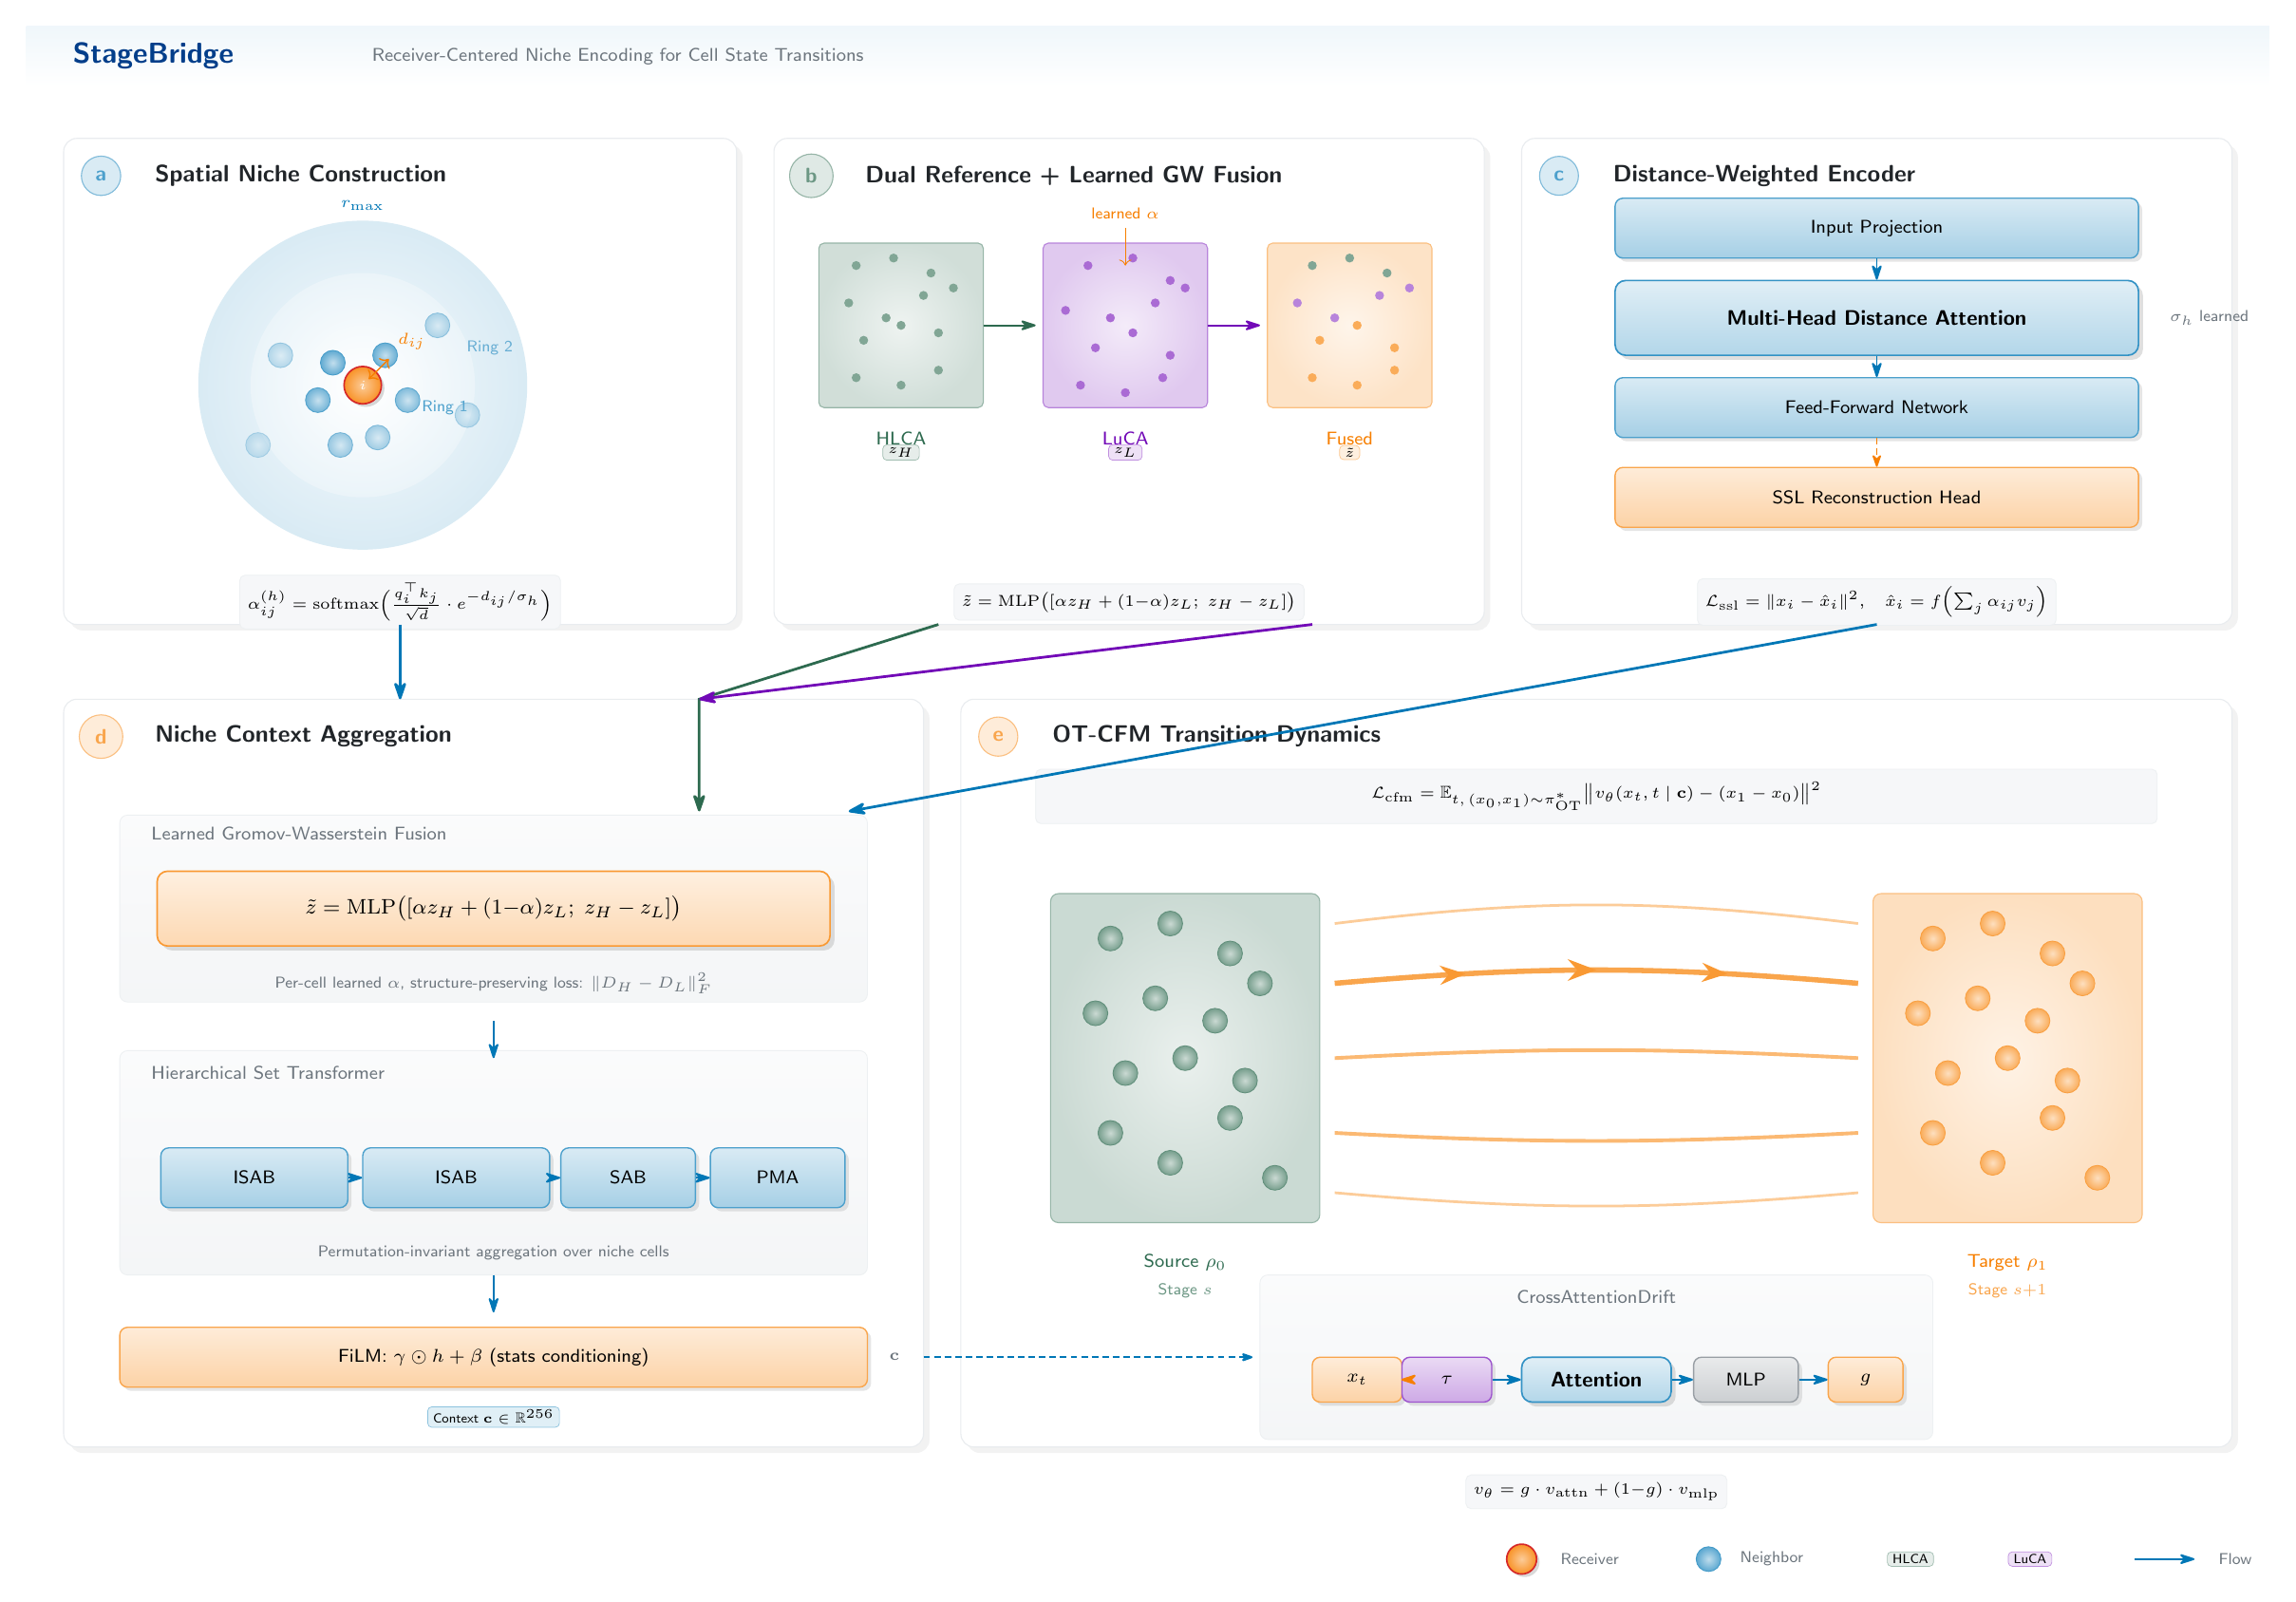
\begin{tikzpicture}[x=1mm, y=1mm]

% ============================================
% CANVAS: 300mm x 200mm (wider for better spacing)
% ============================================
\fill[nbg] (0, 0) rectangle (300, 200);

% Title bar
\shade[top color=nprimary!6, bottom color=nbg] (0, 192) rectangle (300, 200);
\node[font=\fontsize{11}{12}\selectfont\bfseries\sffamily, text=nprimarydk, anchor=west] at (5, 196) {StageBridge};
\node[font=\fontsize{7}{8}\selectfont\sffamily, text=ntextsub, anchor=west] at (45, 196) {Receiver-Centered Niche Encoding for Cell State Transitions};

% ============================================
% ROW 1: PANELS A, B, C (y = 120-185)
% ============================================

% PANEL A: Spatial Niche (x = 5-95)
\node[panel, minimum width=90mm, minimum height=65mm] at (50, 152.5) {};
\node[secletter=nprimary] at (10, 180) {a};
\node[heading, anchor=west] at (16, 180) {Spatial Niche Construction};

\begin{scope}[shift={(45, 152)}]
    % Distance rings (clearer concentric)
    \shade[inner color=nprimary!3, outer color=nprimary!15] (0,0) circle (22mm);
    \shade[inner color=white, outer color=nprimary!8] (0,0) circle (15mm);
    \shade[inner color=white, outer color=nprimary!4] (0,0) circle (8mm);

    % Ring labels
    \node[caption, nprimary] at (0, 24) {$r_{\max}$};
    \node[caption, nprimary!60] at (17, 5) {Ring 2};
    \node[caption, nprimary!70] at (11, -3) {Ring 1};

    % Neighbors (distributed across rings)
    \node[cellsm=nprimary, opacity=0.95] at (-4, 3) {};
    \node[cellsm=nprimary, opacity=0.9] at (3, 4) {};
    \node[cellsm=nprimary, opacity=0.85] at (-6, -2) {};
    \node[cellsm=nprimary, opacity=0.75] at (6, -2) {};
    \node[cellsm=nprimary, opacity=0.6] at (-3, -8) {};
    \node[cellsm=nprimary, opacity=0.55] at (2, -7) {};
    \node[cellsm=nprimary, opacity=0.45] at (10, 8) {};
    \node[cellsm=nprimary, opacity=0.4] at (-11, 4) {};
    \node[cellsm=nprimary, opacity=0.35] at (14, -4) {};
    \node[cellsm=nprimary, opacity=0.3] at (-14, -8) {};

    % Receiver (center, prominent)
    \node[recvcell] at (0, 0) {};
    \node[font=\fontsize{4.5}{5}\selectfont\sffamily, text=white] at (0, 0) {$i$};

    % Distance annotation
    \draw[naccent, line width=0.5pt, <->] (0.8, 0.8) -- (3.5, 3.5);
    \node[caption, naccent, anchor=south west] at (3.5, 3.5) {$d_{ij}$};
\end{scope}

% Equation box for Panel A
\node[eqbox] at (50, 123) {%
    $\alpha_{ij}^{(h)} = \mathrm{softmax}\Bigl(\frac{q_i^\top k_j}{\sqrt{d}} \cdot e^{-d_{ij}/\sigma_h}\Bigr)$
};


% PANEL B: Reference Atlases + GW Fusion (x = 100-195)
\node[panel, minimum width=95mm, minimum height=65mm] at (147.5, 152.5) {};
\node[secletter=ngreen] at (105, 180) {b};
\node[heading, anchor=west] at (111, 180) {Dual Reference + Learned GW Fusion};

% HLCA manifold (left, smaller to make room)
\begin{scope}[shift={(117, 160)}]
    \shade[inner color=ngreen!8, outer color=ngreen!22, rounded corners=2pt]
        (-11, -11) rectangle (11, 11);
    \draw[ngreen!50, line width=0.4pt, rounded corners=2pt] (-11, -11) rectangle (11, 11);

    \foreach \x/\y in {-6/8, -1/9, 4/7, -7/3, -2/1, 3/4, 7/5,
                       -5/-2, 0/0, 5/-1, -6/-7, 0/-8, 5/-6} {
        \fill[ngreen!60] (\x, \y) circle (0.6mm);
    }

    \node[subhead, ngreen, anchor=north] at (0, -13) {HLCA};
    \node[dimbadge=ngreen] at (0, -17) {$z_H$};
\end{scope}

% LuCA manifold (right, smaller)
\begin{scope}[shift={(147, 160)}]
    \shade[inner color=npurple!8, outer color=npurple!22, rounded corners=2pt]
        (-11, -11) rectangle (11, 11);
    \draw[npurple!50, line width=0.4pt, rounded corners=2pt] (-11, -11) rectangle (11, 11);

    \foreach \x/\y in {-5/8, 1/9, 6/6, -8/2, -2/1, 4/3, 8/5,
                       -4/-3, 1/-1, 6/-4, -6/-8, 0/-9, 5/-7} {
        \fill[npurple!60] (\x, \y) circle (0.6mm);
    }

    \node[subhead, npurple, anchor=north] at (0, -13) {LuCA};
    \node[dimbadge=npurple] at (0, -17) {$z_L$};
\end{scope}

% GW Fusion output (fused embedding on far right)
\begin{scope}[shift={(177, 160)}]
    \shade[inner color=naccent!8, outer color=naccent!22, rounded corners=2pt]
        (-11, -11) rectangle (11, 11);
    \draw[naccent!50, line width=0.4pt, rounded corners=2pt] (-11, -11) rectangle (11, 11);

    % Mixed colors to show fusion
    \foreach \x/\y in {-5/8, 0/9, 5/7} {
        \fill[ngreen!60] (\x, \y) circle (0.6mm);
    }
    \foreach \x/\y in {-7/3, -2/1, 4/4, 8/5} {
        \fill[npurple!50] (\x, \y) circle (0.6mm);
    }
    \foreach \x/\y in {-4/-2, 1/0, 6/-3, -5/-7, 1/-8, 6/-6} {
        \fill[naccent!65] (\x, \y) circle (0.6mm);
    }

    \node[subhead, naccent, anchor=north] at (0, -13) {Fused};
    \node[dimbadge=naccent] at (0, -17) {$\tilde{z}$};
\end{scope}

% Fusion arrows
\draw[flowarrow=ngreen] (128, 160) -- (135, 160);
\draw[flowarrow=npurple] (158, 160) -- (165, 160);

% Learned alpha annotation
\node[caption, naccent] at (147, 175) {learned $\alpha$};
\draw[naccent, line width=0.3pt, ->] (147, 173) -- (147, 168);

% GW Fusion equation
\node[eqbox] at (147.5, 123) {%
    $\tilde{z} = \mathrm{MLP}\bigl([\alpha z_H + (1{-}\alpha)z_L;\; z_H - z_L]\bigr)$
};


% PANEL C: Encoder (x = 200-295)
\node[panel, minimum width=95mm, minimum height=65mm] at (247.5, 152.5) {};
\node[secletter=nprimary] at (205, 180) {c};
\node[heading, anchor=west] at (211, 180) {Distance-Weighted Encoder};

\begin{scope}[shift={(247.5, 155)}]
    % Stacked encoder layers
    \node[module3d=nprimary, minimum width=70mm] (proj) at (0, 18) {Input Projection};

    \node[modulebig=nprimary, minimum width=70mm] (attn) at (0, 6) {Multi-Head Distance Attention};
    \node[caption, anchor=west] at (38, 6) {$\sigma_h$ learned};

    \node[module3d=nprimary, minimum width=70mm] (ffn) at (0, -6) {Feed-Forward Network};

    \node[module3d=naccent, minimum width=70mm] (ssl) at (0, -18) {SSL Reconstruction Head};

    \draw[flowarrow=nprimary] (proj) -- (attn);
    \draw[flowarrow=nprimary] (attn) -- (ffn);
    \draw[flowdash=naccent] (ffn) -- (ssl);
\end{scope}

% SSL equation
\node[eqbox] at (247.5, 123) {%
    $\mathcal{L}_{\mathrm{ssl}} = \|x_i - \hat{x}_i\|^2, \quad \hat{x}_i = f\Bigl(\sum_j \alpha_{ij} v_j\Bigr)$
};


% ============================================
% ROW 2: PANELS D, E (y = 10-110)
% ============================================

% PANEL D: Context Refinement (x = 5-120)
\node[panel, minimum width=115mm, minimum height=100mm] at (62.5, 60) {};
\node[secletter=naccent] at (10, 105) {d};
\node[heading, anchor=west] at (16, 105) {Niche Context Aggregation};

% GW Fusion subpanel
\begin{scope}[shift={(62.5, 82)}]
    \node[subpanel, minimum width=100mm, minimum height=25mm] at (0, 0) {};
    \node[subhead, anchor=west] at (-47, 10) {Learned Gromov-Wasserstein Fusion};

    \node[modulebig=naccent, minimum width=90mm] (gw) at (0, 0) {%
        $\tilde{z} = \mathrm{MLP}\bigl([\alpha z_H + (1{-}\alpha)z_L;\; z_H - z_L]\bigr)$
    };

    \node[caption] at (0, -10) {Per-cell learned $\alpha$, structure-preserving loss: $\|D_H - D_L\|_F^2$};
\end{scope}

% Set Transformer subpanel
\begin{scope}[shift={(62.5, 48)}]
    \node[subpanel, minimum width=100mm, minimum height=30mm] at (0, 0) {};
    \node[subhead, anchor=west] at (-47, 12) {Hierarchical Set Transformer};

    \node[module3d=nprimary, minimum width=25mm, minimum height=8mm] (isab1) at (-32, -2) {ISAB};
    \node[module3d=nprimary, minimum width=25mm, minimum height=8mm] (isab2) at (-5, -2) {ISAB};
    \node[module3d=nprimary, minimum width=18mm, minimum height=8mm] (sab) at (18, -2) {SAB};
    \node[module3d=nprimary, minimum width=18mm, minimum height=8mm] (pma) at (38, -2) {PMA};

    \draw[flowarrow=nprimary] (isab1) -- (isab2);
    \draw[flowarrow=nprimary] (isab2) -- (sab);
    \draw[flowarrow=nprimary] (sab) -- (pma);

    \node[caption] at (0, -12) {Permutation-invariant aggregation over niche cells};
\end{scope}

% FiLM conditioning
\begin{scope}[shift={(62.5, 22)}]
    \node[module3d=naccent, minimum width=100mm] (film) at (0, 0) {FiLM: $\gamma \odot h + \beta$ (stats conditioning)};
\end{scope}

\draw[flowarrow=nprimary] (62.5, 67) -- (62.5, 62);
\draw[flowarrow=nprimary] (62.5, 33) -- (62.5, 28);

% Output context
\node[dimbadge=nprimary] at (62.5, 14) {Context $\mathbf{c} \in \mathbb{R}^{256}$};


% PANEL E: Transition Dynamics (x = 125-295)
\node[panel, minimum width=170mm, minimum height=100mm] at (210, 60) {};
\node[secletter=naccent] at (130, 105) {e};
\node[heading, anchor=west] at (136, 105) {OT-CFM Transition Dynamics};

% Source distribution
\begin{scope}[shift={(155, 62)}]
    \shade[inner color=ngreen!10, outer color=ngreen!25, rounded corners=3pt]
        (-18, -22) rectangle (18, 22);
    \draw[ngreen!50, line width=0.4pt, rounded corners=3pt] (-18, -22) rectangle (18, 22);

    \foreach \x/\y in {-10/16, -2/18, 6/14, -12/6, -4/8, 4/5, 10/10,
                       -8/-2, 0/0, 8/-3, -10/-10, -2/-14, 6/-8, 12/-16} {
        \node[cellsm=ngreen] at (\x, \y) {};
    }

    \node[subhead, ngreen, anchor=north] at (0, -25) {Source $\rho_0$};
    \node[caption, ngreen!70, anchor=north] at (0, -29) {Stage $s$};
\end{scope}

% Target distribution
\begin{scope}[shift={(265, 62)}]
    \shade[inner color=naccent!10, outer color=naccent!25, rounded corners=3pt]
        (-18, -22) rectangle (18, 22);
    \draw[naccent!50, line width=0.4pt, rounded corners=3pt] (-18, -22) rectangle (18, 22);

    \foreach \x/\y in {-10/16, -2/18, 6/14, -12/6, -4/8, 4/5, 10/10,
                       -8/-2, 0/0, 8/-3, -10/-10, -2/-14, 6/-8, 12/-16} {
        \node[cellsm=naccent] at (\x, \y) {};
    }

    \node[subhead, naccent, anchor=north] at (0, -25) {Target $\rho_1$};
    \node[caption, naccent!70, anchor=north] at (0, -29) {Stage $s{+}1$};
\end{scope}

% Flow trajectories
\begin{scope}
    \draw[line width=2pt, naccent!70,
        postaction={decorate, decoration={markings,
            mark=at position 0.25 with {\arrow[naccent!80, scale=0.8]{Stealth}},
            mark=at position 0.5 with {\arrow[naccent!80, scale=0.9]{Stealth}},
            mark=at position 0.75 with {\arrow[naccent!80, scale=0.8]{Stealth}}
        }}
    ] (175, 72) to[out=5, in=175] (245, 72);

    \draw[line width=1.4pt, naccent!55] (175, 62) to[out=3, in=177] (245, 62);
    \draw[line width=1.4pt, naccent!55] (175, 52) to[out=-3, in=183] (245, 52);
    \draw[line width=1pt, naccent!40] (175, 80) to[out=7, in=173] (245, 80);
    \draw[line width=1pt, naccent!40] (175, 44) to[out=-5, in=185] (245, 44);
\end{scope}

% CrossAttentionDrift module (compact, below flows)
\begin{scope}[shift={(210, 22)}]
    \node[subpanel, minimum width=90mm, minimum height=22mm] at (0, 0) {};
    \node[subhead] at (0, 8) {CrossAttentionDrift};

    \node[module3d=naccent, minimum width=12mm, minimum height=6mm] (xt) at (-32, -3) {$x_t$};
    \node[module3d=npurple, minimum width=12mm, minimum height=6mm] (tau) at (-20, -3) {$\tau$};
    \node[modulebig=nprimary, minimum width=20mm, minimum height=6mm] (att) at (0, -3) {Attention};
    \node[module3d=ngray, minimum width=14mm, minimum height=6mm] (mlp) at (20, -3) {MLP};
    \node[module3d=naccent, minimum width=10mm, minimum height=6mm] (gate) at (36, -3) {$g$};

    \draw[flowarrow=naccent] (xt) -- (tau);
    \draw[flowarrow=nprimary] (tau) -- (att);
    \draw[flowarrow=nprimary] (att) -- (mlp);
    \draw[flowarrow=nprimary] (mlp) -- (gate);
\end{scope}

% Velocity equation
\node[eqbox] at (210, 4) {%
    $v_\theta = g \cdot v_{\mathrm{attn}} + (1{-}g) \cdot v_{\mathrm{mlp}}$
};

% Loss equation (prominent)
\node[eqbox, minimum width=150mm, inner sep=5pt] at (210, 97) {%
    $\mathcal{L}_{\mathrm{cfm}} = \mathbb{E}_{t,\, (x_0, x_1) \sim \pi^*_{\mathrm{OT}}} \bigl\| v_\theta(x_t, t \mid \mathbf{c}) - (x_1 - x_0) \bigr\|^2$
};

% Context arrow
\draw[flowdash=nprimary, line width=0.8pt] (120, 22) -- (164, 22);
\node[caption, anchor=east] at (118, 22) {$\mathbf{c}$};


% ============================================
% INTER-PANEL ARROWS (Row 1 to Row 2)
% ============================================
% A -> D (spatial niche input)
\draw[flowthick=nprimary] (50, 120) -- (50, 110);

% B -> D (reference embeddings)
\draw[flowthick=ngreen] (122, 120) -- (90, 110) -- (90, 95);
\draw[flowthick=npurple] (172, 120) -- (90, 110);

% C -> D (niche embeddings)
\draw[flowthick=nprimary] (247.5, 120) -- (110, 95);


% ============================================
% LEGEND (bottom right)
% ============================================
\begin{scope}[shift={(200, -5)}]
    \node[recvcell, minimum size=4mm] at (0, 0) {};
    \node[caption, anchor=west] at (4, 0) {Receiver};

    \node[cellsm=nprimary] at (25, 0) {};
    \node[caption, anchor=west] at (28, 0) {Neighbor};

    \node[dimbadge=ngreen] at (52, 0) {HLCA};
    \node[dimbadge=npurple] at (68, 0) {LuCA};

    \draw[flowarrow=nprimary] (82, 0) -- (90, 0);
    \node[caption, anchor=west] at (92, 0) {Flow};
\end{scope}

\end{tikzpicture}

\end{document}
